%
% 04_verallgemeinerung.tex -- Verallgemeinerung des Jordan'schen Kurventheorems
%
% (c) 2026 Dominik Castelberg, Ostschweizer Fachhochschule
%
% !TEX root = ../../buch.tex
% !TEX encoding = UTF-8
%
\section{Verallgemeinerung des Satzes von Jordan
\label{jordan:section:teil3}}
\kopfrechts{Teil 3}

\subsection{Die Alexander-Dualität
\label{jordan:subsection:alexander}}

\begin{figure}
    \centering
    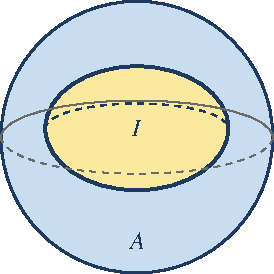
\includegraphics{papers/jordan/images/alexander_dualitaet.pdf}
    \caption{Geometrische Zerlegung der Alexander-Dualität.}
\end{figure}


\subsection{Der Jordan-Brouwer-Zerlegungssatz
\label{jordan:subsection:jordanbrouwer}}

\begin{figure}
    \centering
    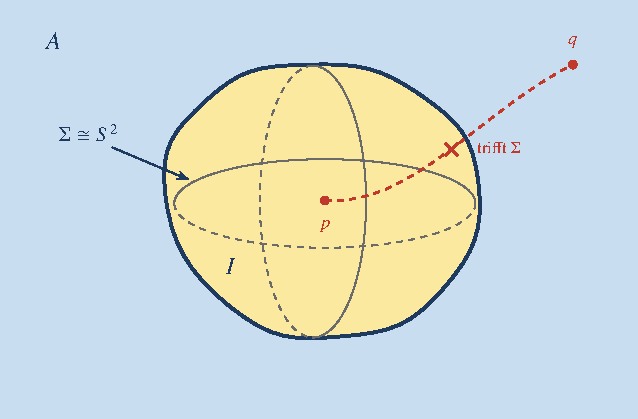
\includegraphics{papers/jordan/images/jordan_brouwer.pdf}
    \caption{Visualisierung des Jordan-Brouwer-Zerlegungssatzes im 3-dimensionalen Raum. $\mathbb{R}^{3}\setminus\Sigma$ zerfällt in genau zwei Komponenten: $\mathrm{I}$ beschränkt, $\mathrm{A}$ unbeschränkt}
\end{figure}

